%\newcommand{\FigInc}{%
%\begin{wrapfigure}{R}{3.05in}
%  \begin{mdframed}
%  \includegraphics[width=3.0in]{./Figures/Figure.pdf}
%  \caption{An example figure with caption to explain.}
%  \label{incFigure}
%  \end{mdframed}
%\end{wrapfigure}}


\subsubsection{Aim 1: \SpecificAimOne}

\paragraph{Introduction}

Aim 1 focuses on preprocessing the raw genomic data collected from Black Americans with NSCLC. 
This process is essential for ensuring the accuracy and reliability of subsequent analyses. 
Given the complexity and volume of genomic data, meticulous preprocessing is required to remove biases, correct errors, 
and prepare the data for detailed mutation and evolutionary analysis. 

\begin{figure}[h] % "htbp" here means "here, top, bottom, or on a float page", controlling where the figure is placed
  \centering
  \begin{mdframed}
  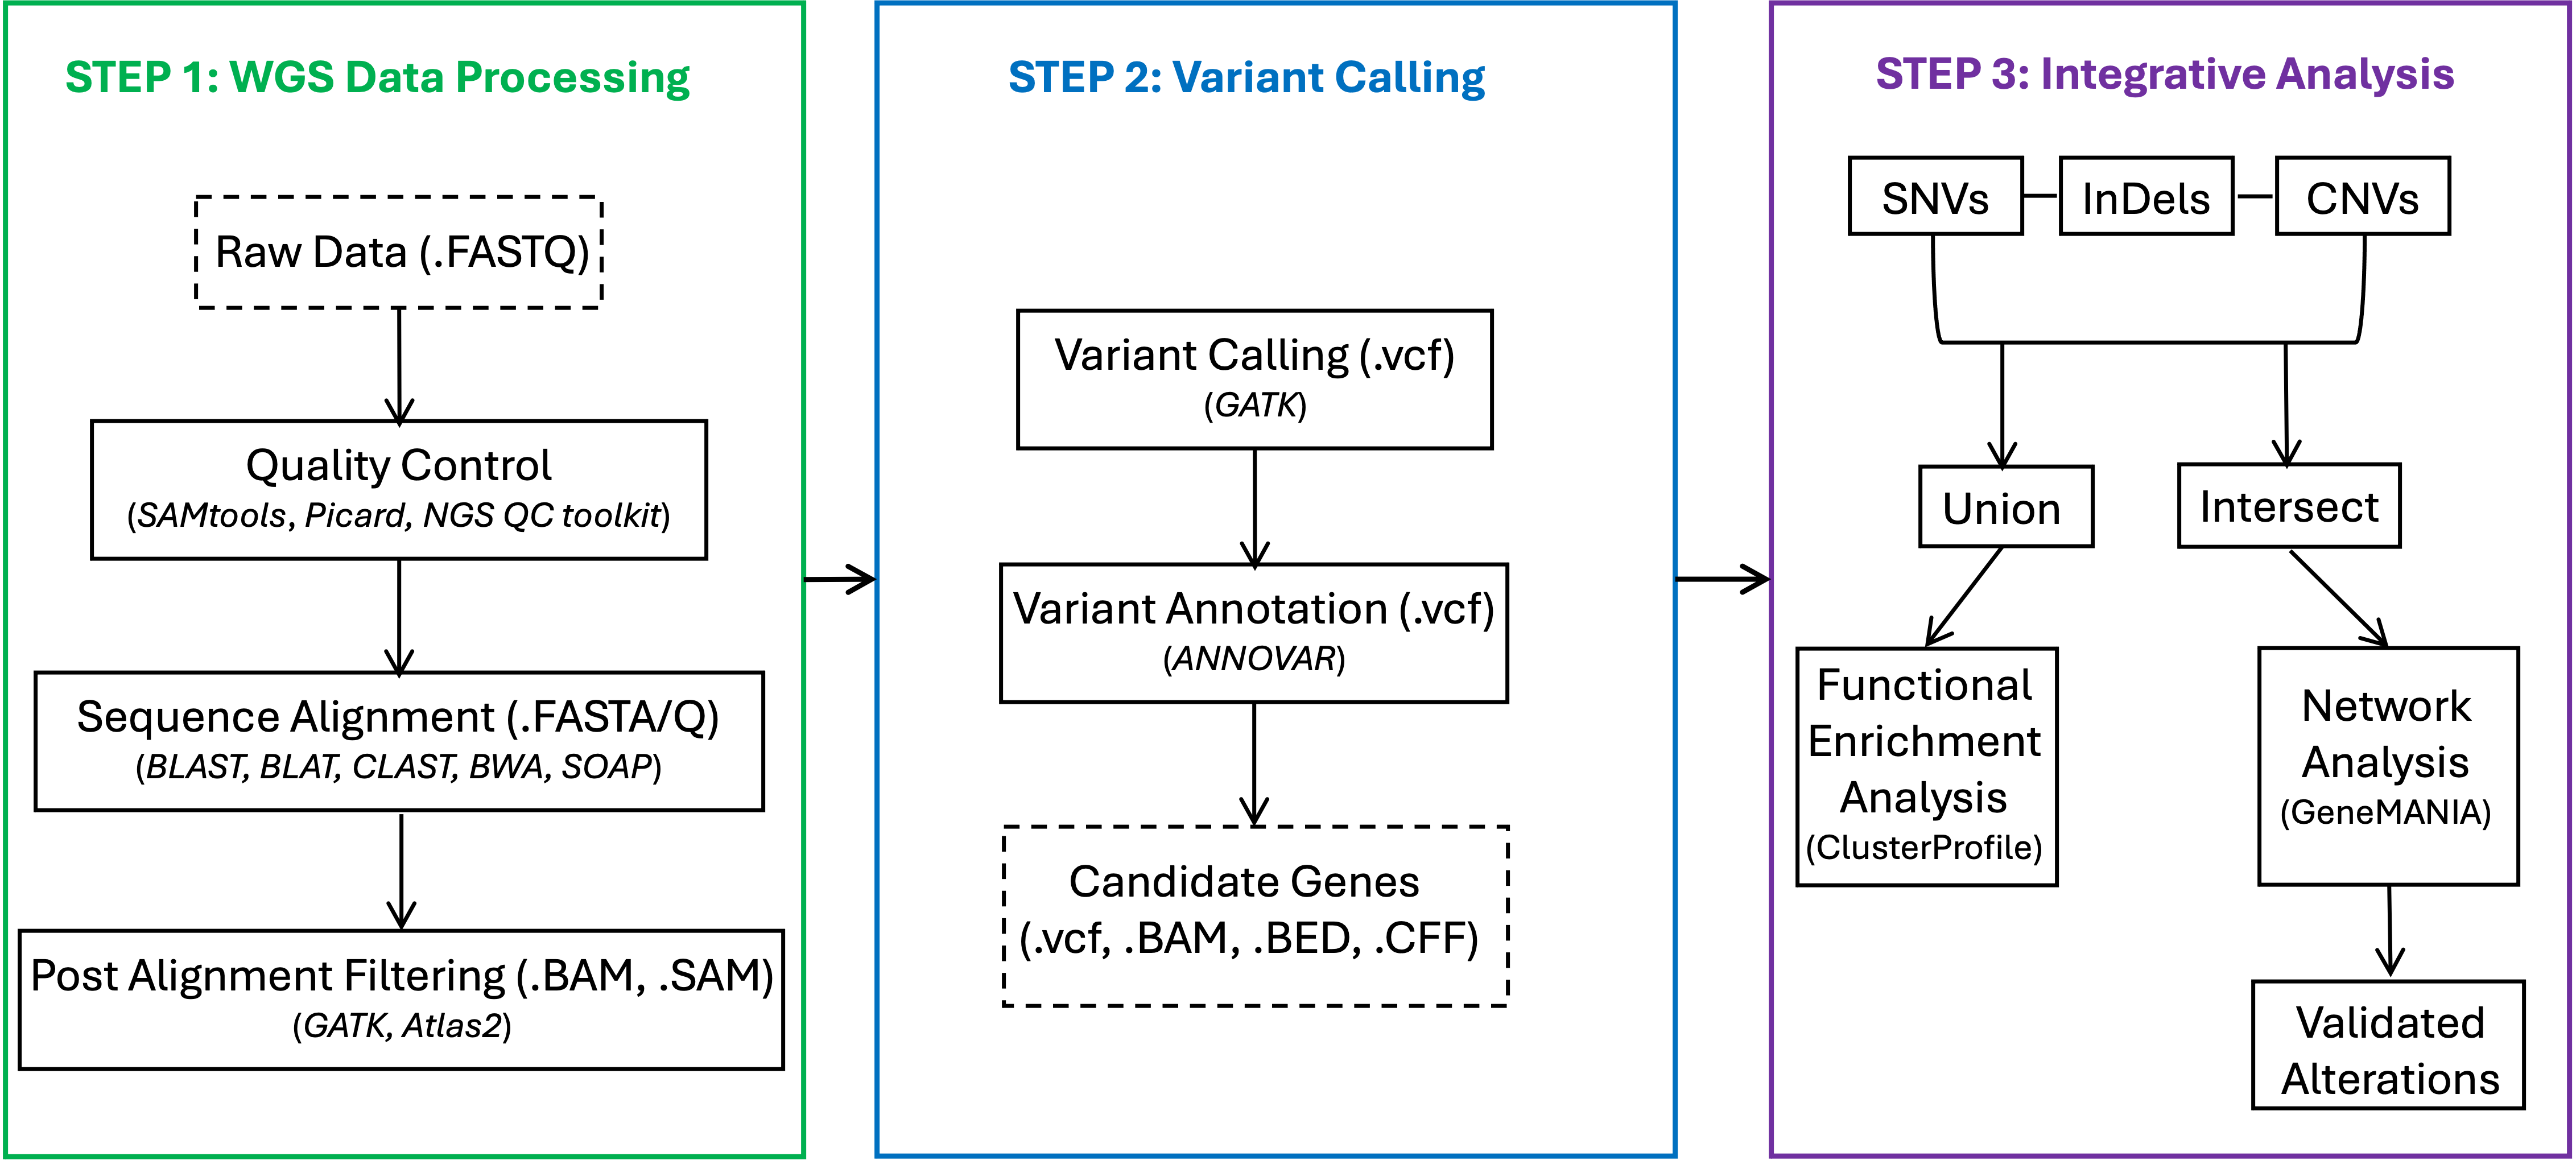
\includegraphics[width=7.4in]{./Figures/data-processing.png}
  \caption{Standard pipeline for NGS analysis.
  STEP 1: Raw data (FASTQ) are aligned to the reference data (FASTA). Resulting alignments are stored in binary alignment map (BAM) file format. 
  STEP 2: Sequence variants are identified and annotated using tools such as GATK and ANNOVAR. Candidate genes are stored in various file formats, \textit{e.g.} .vcf, .BAM, .BED, .CFF.
  STEP 3: Candidate genes with SNVs, InDels, and CNVs are analyzed and validated using tools such as ClusterProfile and GeneMANIA.
  }
  \label{data-processing}
  \end{mdframed}
\end{figure}

\vspace{1em}
\noindent
Whole genome sequencing (WGS) is a comprehensive method for analyzing the entire genomic DNA of an organism. 
This technique allows for the identification of genetic variations, including single nucleotide variants (SNVs), 
insertions and/or deletions (InDels), and structural variations across the entire genome. 
Next-generation sequencing (NGS) refers to a collection of modern sequencing technologies that enable the rapid sequencing of large amounts of DNA. 
These technologies have revolutionized genomic research by providing high-throughput, accurate, and cost-effective sequencing solutions.~\cite{koboldt_best_2020-1} 
NGS allows for easy implementation of WGS, providing a powerful framework for uncovering the genetic underpinnings of diseases such as NSCLC.

\vspace{1em}
\noindent
Given the nature of genomic data, which often contains significant amounts of noise due to sequencing processes, 
a series of rigorous data cleaning protocols is commonly implemented. 
This includes removing low-quality sequences to prevent erroneous interpretations, 
aligning the raw reads to a reference genome to identify the genomic coordinates of the sequences, 
removing duplicate reads to avoid overrepresentation, and correcting sequencing errors to improve data accuracy. 
Additionally, it is crucial to account for mutations present in healthy cells to differentiate between 
somatic mutations and germline variants, thus focusing on cancer-specific changes.~\cite{koboldt_best_2020-1,gerstung_evolutionary_2020}

\vspace{1em}
\noindent
Once the data has been cleaned, the next step is normalization. 
Genomic data can be affected by various technical variances and batch effects that arise during sample collection, sequencing, and processing. 
These variances can obscure true biological signals if not properly addressed.~\cite{jaffe_practical_2015} 
The normalization process involves adjusting for systematic biases and standardizing the data to 
ensure that it is comparable across different samples and experimental conditions. 
This is particularly important when dealing with large datasets collected from diverse sources, 
as it enhances the comparability of the data and ensures that any observed differences 
are due to biological variations rather than technical artifacts.

\vspace{1em}
\noindent
The final preprocessing step involves the detection and classification of mutations. This step is crucial for understanding the genetic underpinnings of NSCLC and involves identifying single nucleotide variants (SNVs), which are point mutations that can significantly impact gene function, as well as detecting insertions and deletions (indels) that result in structural genomic changes. Additionally, it is essential to identify and analyze copy number variants (CNVs), which are large regions of the genome that have been duplicated or deleted. CNVs can have significant implications for gene expression and tumor progression. Using established bioinformatics pipelines to classify and annotate these genetic variations provides insights into their potential impact and relevance to cancer progression. By accurately detecting and classifying these mutations and CNVs, we can create a comprehensive genetic profile of NSCLC in Black Americans, which serves as a foundation for further evolutionary analyses \cite{gerstung_evolutionary_2020}.

\vspace{1em}
\noindent
We anticipate several challenges in this aim, including high inter-individual variability in mutation rates and evolutionary patterns. 
To address these challenges, we plan to incorporate a larger sample size to mitigate the impact of individual variability and provide more robust statistical power. 
Employing advanced statistical techniques will help ensure that our findings are generalizable and reliable. 
The computational demands of methods like GRITIC will be managed by leveraging high-performance computing resources, ensuring that analyses are conducted efficiently and accurately. 
Additionally, using standardized data formats and developing custom scripts for data merging and analysis will facilitate the seamless integration of results from different computational methods (Gerstung et al., 2020).

\paragraph{Rationale}

Aim 1 focuses on preprocessing the raw genomic data from Black Americans diagnosed with NSCLC, 
a demographic often underrepresented in cancer research. 
This step is crucial for establishing a reliable baseline for subsequent analyses. 
By implementing rigorous data cleaning and preprocessing protocols, we aim to remove low-quality sequences, 
align the reads to the reference genome, and filter data for further analysis using \texttt{GRITIC}. 
The resulting high-quality dataset will be essential for accurately mapping mutational signatures and evolutionary patterns specific to this population.

%\begin{wrapfigure}{R}{2.05in}
%  \begin{mdframed}
%  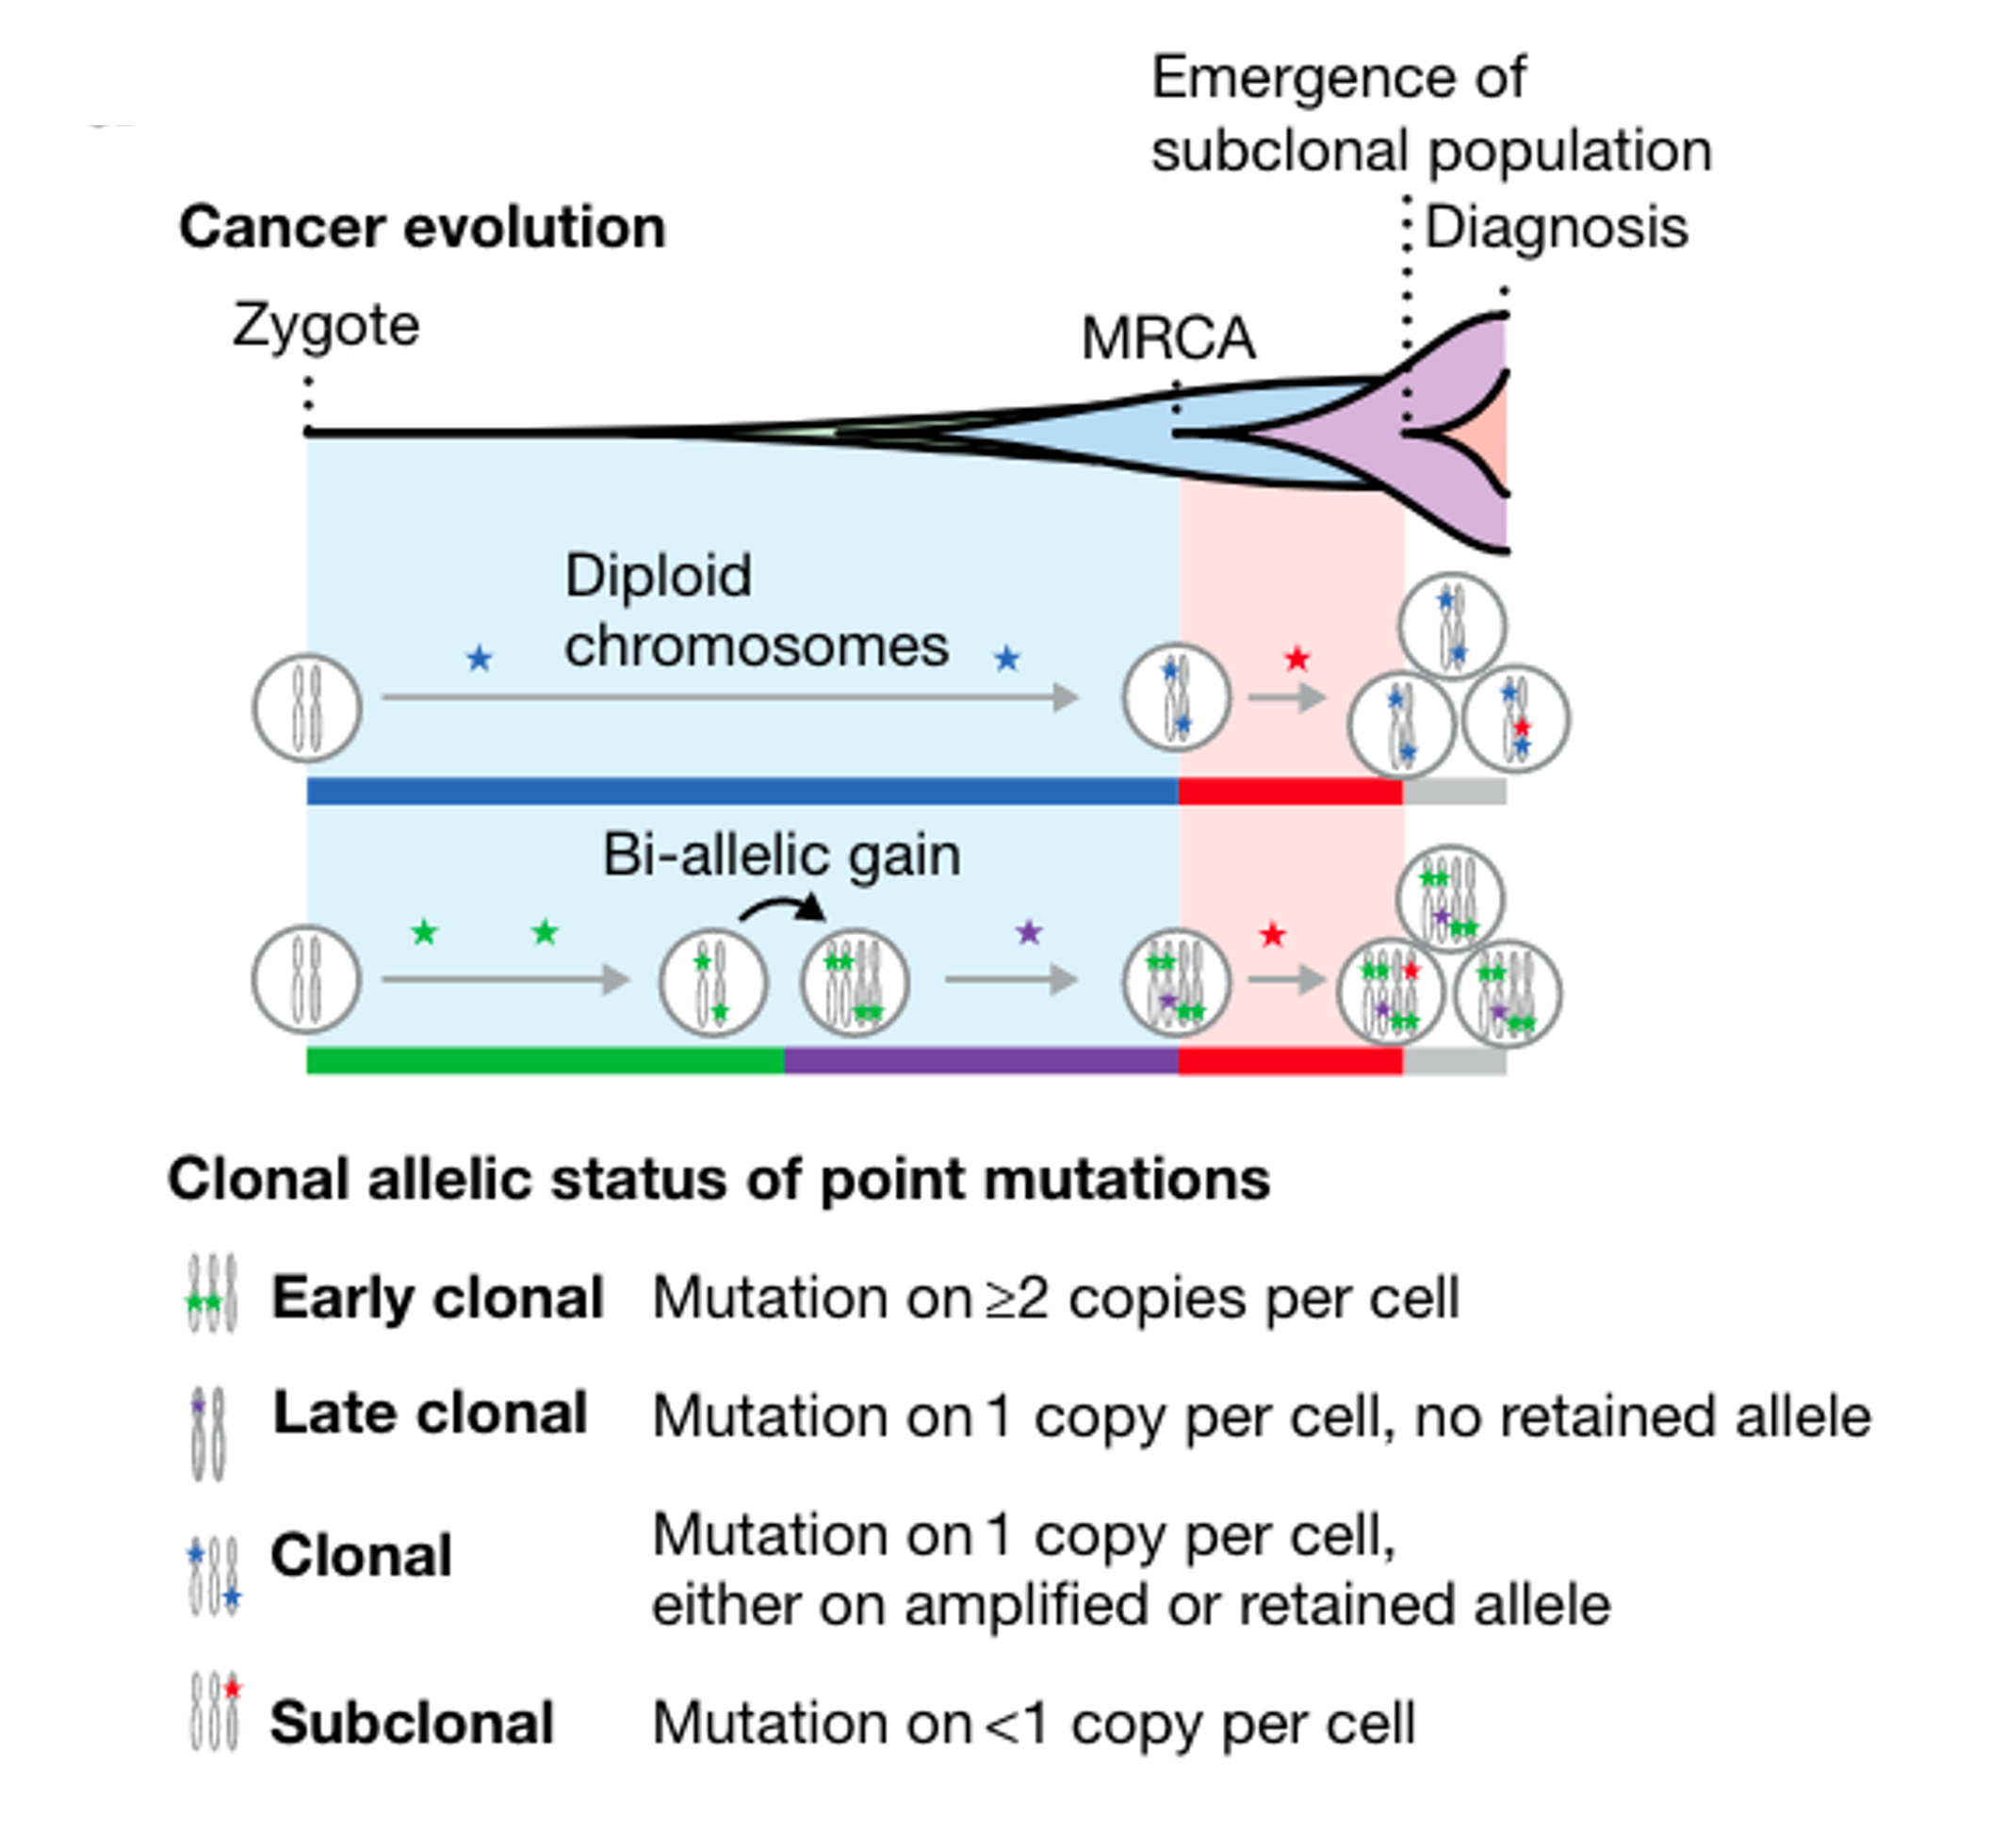
\includegraphics[width=2.0in]{./Figures/definitions.png}
%  \caption{Principles of timing mutations and copy number gains based on whole-genome sequencing. 
%  Figure from Gerstung \textit{et al.}
%  }
%  \label{definitions}
%  \end{mdframed}
%\end{wrapfigure}


\paragraph{1.1. \SpecificAimOneA}

This stage involves collaborating with regional medical centers and cancer research networks to collect extensive genomic data from NSCLC patients, particularly those of Black American descent. The data will undergo rigorous cleaning and preprocessing steps to remove biases and errors. This includes aligning sequences to reference genomes, removing duplicate reads, correcting sequencing errors, and accounting for mutations in healthy cells. We will implement stringent quality control measures to validate the data's integrity and completeness, ensuring it meets the analytical requirements of the computational methods to be applied. This step is expected to be time-consuming, given the complexity of preprocessing genomic data.

\paragraph{1.2. \SpecificAimOneB}

In this phase, we will normalize the dataset to account for batch effects and other technical variances. Normalization is crucial to ensure that the data is comparable across different samples and experiments. This involves adjusting for systematic biases that may arise during data collection and sequencing processes. We will employ robust statistical techniques to standardize the data, making it suitable for downstream analyses such as mutation detection and evolutionary trajectory modeling.

\paragraph{1.3. \SpecificAimOneC}

After normalizing the data, we will detect and classify mutations, including single nucleotide variants (SNVs), insertions, and deletions, using established bioinformatics pipelines. These pipelines will enable us to systematically identify and annotate genetic variations within the dataset. The accurate detection and classification of mutations are critical for subsequent evolutionary analyses, as they provide the foundation for understanding the genetic dynamics and progression of NSCLC in this population.

%\begin{wrapfigure}{R}{4.05in}
%  \begin{mdframed}
%  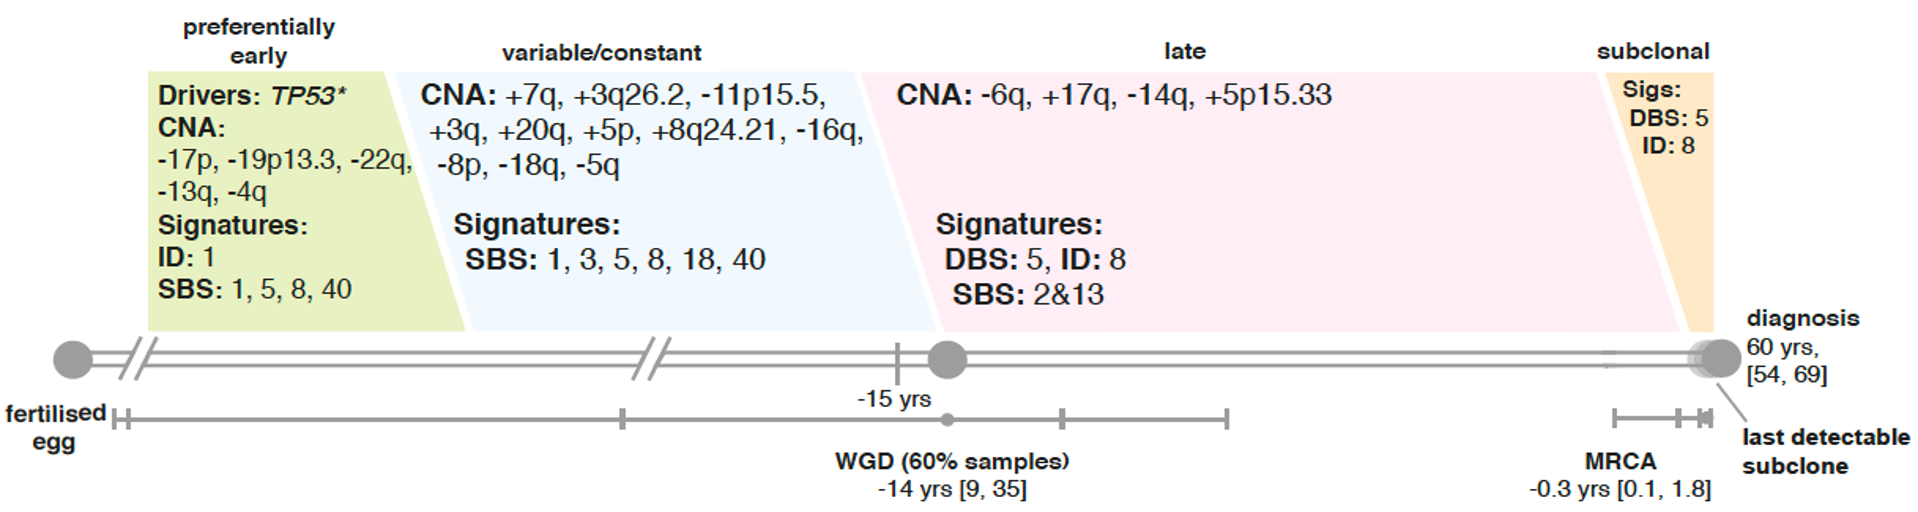
\includegraphics[width=4.0in]{./Figures/evolution-map.png}
%  \caption{Timing model for serous ovarian carcinomas. 
%  			Estimates on when major events occur during tumor development are provided.~\cite{gerstung_evolutionary_2020}}
%  \label{timeline}
%  \end{mdframed}
%\end{wrapfigure}

\paragraph{Challenges \& Alternative Approaches}

We anticipate challenges such as high inter-individual variability in mutation rates and evolutionary patterns. To address this, we plan to incorporate a larger sample size and employ robust statistical methods to ensure the generalizability of our findings. The computational demands of the \texttt{GRITIC} method will be managed by leveraging high-performance computing resources and optimizing algorithm parameters to enhance computational efficiency without compromising accuracy. We will also ensure seamless integration of results from different computational methods by using standardized data formats and developing custom scripts for data merging and analysis.